\documentclass[border=8pt, multi, crop, tikz]{standalone}
%\usepackage{blocks}
% \usepackage[top=4cm,left=2cm]{geometry}
\usepackage{import}
\subimport{/home/thesis/PlotNeuralNets/layers/}{init}
\usetikzlibrary{positioning}
\usetikzlibrary{3d} %for including external image 

\def\ConvColor{rgb:yellow,5;red,2.5;white,5}
\def\ConvReluColor{rgb:yellow,5;red,5}
\def\PoolColor{rgb:red,1;black,0}
\def\UnpoolColor{rgb:blue,2;green,1;black,0.3}
\def\FcColor{rgb:blue,5;red,2.5;white,5}
\def\FcReluColor{rgb:blue,5;red,5;white,4}
\def\SoftmaxColor{rgb:magenta,5;black,7}
\def\SumColor{rgb:blue,5;green,15}
\def\LayerColor{rgb:black,1}


\newcommand{\copymidarrow}{\tikz \draw[-Stealth,line width =0.8mm,draw={rgb:blue,4;red,1;green,1;black,3}] (-0.3,0) -- ++(0.3,0);}


\begin{document}
\noindent
\begin{tikzpicture}
	\tikzstyle{connection}=[ultra thick,every node/.style={sloped,allow upside down},draw=\edgecolor,opacity=0.7]
	\tikzstyle{copyconnection}=[ultra thick,every node/.style={sloped,allow upside down},draw={rgb:blue,4;red,1;green,1;black,3},opacity=0.7]

	%%%%%%%%%%%%%%%%%%%%%%%%%%%%%%%%%%%%%%%%%%%%%%%%%%%%%%%%%%%%%%%%%%%%%%%%%%%%%%%%%%%%%%%%
	%% Draw Encoder
	%%%%%%%%%%%%%%%%%%%%%%%%%%%%%%%%%%%%%%%%%%%%%%%%%%%%%%%%%%%%%%%%%%%%%%%%%%%%%%%%%%%%%%%%
	% input picture
	\node[canvas is zy plane at x=0] (temp) at (-3.5,0,0) {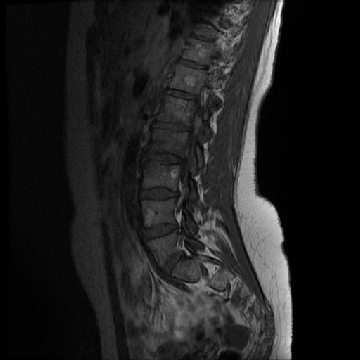
\includegraphics[width=-8cm,height=8cm]{/home/thesis/PlotNeuralNets/images/input.png}};
	\path (-5,0,0);
	% input
	\pic[shift={(0,0,0)}] at (0,0,0) {
		Box={
				name=input,
				caption=Input,
				xlabel={{"1","28"}},
				ylabel=28,
				zlabel=28,
				fill=\ConvColor,
				height=28,
				width=0.09375,
				depth=28
			}
	};
	% conv1
	\pic[shift={(1.5,0,0)}] at (input-east) {
		RightBandedBox={
				name=conv1,
				caption=Conv1\\3\(\times\)3,
				xlabel={{"16",""}},
				ylabel=28,
				fill=\ConvColor,
				bandfill=\ConvReluColor,
				height=28,
				width=1.5,
				depth=28
			}
	};

	% layer1
	% res1_1_1
	\pic[shift={(1.5,0,0)}] at (conv1-east) {
		RightBandedBox={
				name=res1_1_1,
				xlabel={{"16",""}},
				ylabel=28,
				fill=\ConvColor,
				bandfill=\ConvReluColor,
				height=28,
				width=1.5,
				depth=28
			}
	};
	% res1_1_2
	\pic[shift={(0,0,0)}] at (res1_1_1-east) {
		Box={
				name=res1_1_2,
				caption=\makebox[0pt]{\shortstack[c]{3\(\times\)3 bn relu\\3\(\times\)3\\ele\_add bn relu}},
				xlabel={{"16",""}},
				zlabel=28,
				fill=\ConvColor,
				height=28,
				width=1.5,
				depth=28
			}
	};
	% add1_1
	\pic[shift={(0,0,0)}] at (res1_1_2-east) {
		Ball={
				name=add1_1,
				fill=\SumColor,
				opacity=0.6,
				radius=2.5,
				logo=\(+\)
			}
	};
	% relu1_1
	\pic[shift={(0,0,0)}] at (add1_1-east) {
		Box={
				name=relu1_1,
				caption=,
				xlabel={{"16",""}},
				zlabel=28,
				fill=\ConvReluColor,
				height=28,
				width=1.5,
				depth=28
			}
	};

	% res1_2_1
	\pic[shift={(1.5,0,0)}] at (relu1_1-east) {
		RightBandedBox={
				name=res1_2_1,
				xlabel={{"16",""}},
				ylabel=28,
				fill=\ConvColor,
				bandfill=\ConvReluColor,
				height=28,
				width=1.5,
				depth=28
			}
	};
	% res1_2_2
	\pic[shift={(0,0,0)}] at (res1_2_1-east) {
		Box={
				name=res1_2_2,
				caption=\makebox[0pt]{\shortstack[c]{3\(\times\)3 bn relu\\3\(\times\)3\\ele\_add bn relu}},
				xlabel={{"16",""}},
				zlabel=28,
				fill=\ConvColor,
				height=28,
				width=1.5,
				depth=28
			}
	};
	% add1_2
	\pic[shift={(0,0,0)}] at (res1_2_2-east) {
		Ball={
				name=add1_2,
				fill=\SumColor,
				opacity=0.6,
				radius=2.5,
				logo=\(+\)
			}
	};
	% relu1_2
	\pic[shift={(0,0,0)}] at (add1_2-east) {
		Box={
				name=relu1_2,
				caption=,
				xlabel={{"16",""}},
				zlabel=28,
				fill=\ConvReluColor,
				height=28,
				width=1.5,
				depth=28
			}
	};

	% res1_3_1
	\pic[shift={(1.5,0,0)}] at (relu1_2-east) {
		RightBandedBox={
				name=res1_3_1,
				xlabel={{"16",""}},
				ylabel=28,
				fill=\ConvColor,
				bandfill=\ConvReluColor,
				height=28,
				width=1.5,
				depth=28
			}
	};
	% res1_3_2
	\pic[shift={(0,0,0)}] at (res1_3_1-east) {
		Box={
				name=res1_3_2,
				caption=\makebox[0pt]{\shortstack[c]{3\(\times\)3 bn relu\\3\(\times\)3\\ele\_add bn relu}},
				xlabel={{"16",""}},
				zlabel=28,
				fill=\ConvColor,
				height=28,
				width=1.5,
				depth=28
			}
	};
	% add1_3
	\pic[shift={(0,0,0)}] at (res1_3_2-east) {
		Ball={
				name=add1_3,
				fill=\SumColor,
				opacity=0.6,
				radius=2.5,
				logo=\(+\)
			}
	};
	% relu1_3
	\pic[shift={(0,0,0)}] at (add1_3-east) {
		Box={
				name=relu1_3,
				caption=,
				xlabel={{"16",""}},
				zlabel=28,
				fill=\ConvReluColor,
				height=28,
				width=1.5,
				depth=28
			}
	};


	% layer2
	% res2_1_1
	\pic[shift={(1.5,0,0)}] at (relu1_3-east) {
		RightBandedBox={
				name=res2_1_1,
				xlabel={{"32",""}},
				ylabel=28,
				fill=\ConvColor,
				bandfill=\ConvReluColor,
				height=28,
				width=3,
				depth=28
			}
	};
	% warp2
	\pic[shift={(1.5,7,0)}] at (relu1_3-east) {
		Box={
				name=warp2,
				caption=\makebox[0pt]{\shortstack[c]{1\(\times\)1}},
				xlabel={{"32",""}},
				ylabel=28,
				fill=\UnpoolColor,
				height=28,
				width=3,
				depth=28
			}
	};
	% res2_1_2
	\pic[shift={(0,0,0)}] at (res2_1_1-east) {
		Box={
				name=res2_1_2,
				caption=\makebox[0pt]{\shortstack[c]{3\(\times\)3 bn relu\\3\(\times\)3\\ele\_add bn relu}},
				xlabel={{"32",""}},
				zlabel=28,
				fill=\ConvColor,
				height=28,
				width=3,
				depth=28
			}
	};
	% add2_1
	\pic[shift={(0,0,0)}] at (res2_1_2-east) {
		Ball={
				name=add2_1,
				fill=\SumColor,
				opacity=0.6,
				radius=2.5,
				logo=\(+\)
			}
	};
	% relu2_1
	\pic[shift={(0,0,0)}] at (add2_1-east) {
		Box={
				name=relu2_1,
				caption=,
				xlabel={{"32",""}},
				zlabel=28,
				fill=\ConvReluColor,
				height=28,
				width=3,
				depth=28
			}
	};

	% pool2d
	\pic[shift={(1.5,0,0)}] at (relu2_1-east) {
		Box={
				name=pool2d,
				caption=\makebox[0pt]{\shortstack[c]{avg\_pool\\size=8\\stride=1}},
				xlabel={{"128",""}},
				ylabel=23,
				zlabel=23,
				fill=\PoolColor,
				height=23,
				width=12,
				depth=23
			}
	};

	% fullconnection
	\pic[shift={(1.5,0,0)}] at (pool2d-east) {
		RightBandedBox={
				name=fc,
				caption=\makebox[0pt]{\shortstack[c]{full\_connection\\softmax}},
				xlabel={{"1",""}},
				zlabel=10,
				fill=\FcColor,
				bandfill=\SoftmaxColor,
				height=4,
				width=4,
				depth=40
			}
	};

	% connections
	\draw [connection]  		(input-east)			-- 	node {\midarrow} 	(conv1-west);
	\draw [connection]  		(conv1-east)			-- 	node {\midarrow} 	(res1_1_1-west);
	\draw [connection]  		(relu1_1-east)			-- 	node {\midarrow} 	(res1_2_1-west);
	\draw [connection]  		(relu1_2-east)			-- 	node {\midarrow} 	(res1_3_1-west);
	\draw [connection]  		(relu1_3-east)			-- 	node {\midarrow} 	(res2_1_1-west);


	% connections shortcut
	% conv1 to add1_1
	\path (add1_1-north) ++ (0,4,0) coordinate (add1_1-north-above);
	\draw [connection] (conv1-north) -- node {\midarrow} (conv1-north|-add1_1-north-above) -- node {\midarrow} (add1_1-north-above) -- node {\midarrow} (add1_1-north);
	% relu1_1 to add1_2
	\path (add1_2-north) ++ (0,4,0) coordinate (add1_2-north-above);
	\draw [connection] (relu1_1-north) -- node {\midarrow} (relu1_1-north|-add1_2-north-above) -- node {\midarrow} (add1_2-north-above) -- node {\midarrow} (add1_2-north);
	% relu1_2 to add1_3
	\path (add1_3-north) ++ (0,4,0) coordinate (add1_3-north-above);
	\draw [connection] (relu1_2-north) -- node {\midarrow} (relu1_2-north|-add1_3-north-above) -- node {\midarrow} (add1_3-north-above) -- node {\midarrow} (add1_3-north);

	% relu1_3 to warp2_1
	\draw [connection] (relu1_3-north) -- node {\midarrow} (relu1_3-north|-warp2-west) -- node {\midarrow} (warp2-west);
	\draw [connection] (warp2-east) -- node {\midarrow} (warp2-east-|add2_1-north) -- node {\midarrow} (add2_1-north);


	% pool & fullconnection
	\draw	[densely dashed]  (relu2_1-nearnortheast)    	--  									(pool2d-nearnorthwest);
	\draw	[densely dashed]  (relu2_1-nearsoutheast)    	--  									(pool2d-nearsouthwest);
	\draw	[densely dashed]  (relu2_1-farnortheast)    	--  									(pool2d-farnorthwest);
	\draw	[densely dashed]  (relu2_1-farsoutheast)    	--  									(pool2d-farsouthwest);

	\draw	[densely dashed]  (pool2d-nearnortheast)    	--  									(fc-nearnorthwest);
	\draw	[densely dashed]  (pool2d-nearsoutheast)    	--  									(fc-nearsouthwest);
	\draw	[densely dashed]  (pool2d-farnortheast)    	--  									(fc-farnorthwest);
	\draw	[densely dashed]  (pool2d-farsoutheast)    	--  									(fc-farsouthwest);
	%%%%%%%%%%%%%%%%%%%%%%%%%%%%%%%%%%%%%%%%%%%%%%%%%%%%%%%%%%%%%%%%%%%%%%%%%%%%%%%%%%%%%%%
\end{tikzpicture}
\end{document}
